\documentclass{article}
\pagestyle{empty}

\usepackage[a3paper,landscape,margin=1cm]{geometry}
%\usepackage{showframe} % DO NOT COMBINE WITH TIKZexternalize

\usepackage{tikz}

% \usepackage{etoolbox}

%Set/get variables, see https://tex.stackexchange.com/a/37113
\usepackage{pgfkeys}
\newcommand{\setvalue}[1]{\pgfkeys{/variables/#1}}
\newcommand{\getvalue}[1]{\pgfkeysvalueof{/variables/#1}}
\newcommand{\declare}[1]{%
  \pgfkeys{
    /variables/#1.is family,
    /variables/#1.unknown/.style = {\pgfkeyscurrentpath/\pgfkeyscurrentname/.initial = ##1}
  }%
}
\declare{} %Setup the /variables directory

% set up externalization (COMMENT OUT FOR DEBUGGING!)
\usetikzlibrary{external}
\tikzexternalize[prefix=./outputLayout_unbroken/]

% load macros
%% TIKZ MACROS to generate beamline layouts
%% TO BE INCLUDED INTO A LATEX DOCUMENT
%% K. Sjobak, 2018

\usepackage{calc}

\newcommand{\belemsiz}{\footnotesize}

% ARG 1: X pos
% ARG 2: text
\newcommand{\correctorMagnet}[2]{
    \filldraw[blue!80] (#1,0) -- (#1-0.15, 0.35) -- (#1+0.15, 0.35);
    \filldraw[blue!80] (#1,0) -- (#1-0.15,-0.35) -- (#1+0.15,-0.35);

    \if\getvalue{elemnames}1
        \node[rotate=-90,anchor=west] at (#1,-0.7) {\belemsiz #2};
    \fi
}

% ARG 1: Y pos (default = 0.0)
% ARG 2: X pos
% ARG 3: text
\newcommand{\BTV}[3][0.0]{
    \draw[ultra thick, purple] (#2,#1) circle (0.3);
    \draw[ultra thick, purple] (#2,#1-0.2) -- (#2,#1+0.2);

    \if\getvalue{elemnames}1
        \node[rotate=-90,anchor=west,align=left] at (#2,#1-0.7) {\belemsiz #3};
    \fi
}

% ARG 1: Y pos (default = 0.0)
% ARG 2: X pos
% ARG 3: text
% ARG 4: radius
\newcommand{\cBPM}[4][0.0]{
    \draw[ultra thick, purple] (#2,#1) circle (#4);

    \if\getvalue{elemnames}1
        \node[rotate=-90,anchor=west] at (#2,#1-0.7) {\belemsiz #3};
    \fi
}

% ARG 1: Y pos (default = 0.0)
% ARG 2: X pos
% ARG 3: text
\newcommand{\iBPM}[3][0.0]{
    \draw[ultra thick, purple] ({#2-0.15},#1-0.15) rectangle ({#2+0.15},#1+0.15);

    \if\getvalue{elemnames}1
        \node[rotate=-90,anchor=west] at (#2,#1-0.7) {\belemsiz #3};
    \fi
}

% ARG 1: Color (default = blue!50)
% ARG 2: X pos
% ARG 3: text
\newcommand{\lensF}[3][blue!50] {
    \pgfmathsetmacro{\lensRadius}{2};
    \pgfmathsetmacro{\lensHeight}{0.7};
    \pgfmathsetmacro{\startAngle}{asin(\lensHeight/\lensRadius)};

    \draw [fill=#1]  (#2,\lensHeight)
         arc[start angle=180-\startAngle,delta angle=2*\startAngle,radius=\lensRadius]
         arc[start angle=-\startAngle,delta angle=2*\startAngle,radius=\lensRadius]
         -- cycle; % to get a better line end

    \if\getvalue{elemnames}1
       \node[rotate=-90,anchor=west,align=left] at (#2,-0.7) {\belemsiz #3};
    \fi
}

% ARG 1: X pos
% ARG 2: text
\newcommand{\lensD}[2] {
    \pgfmathsetmacro{\lensRadius}{2};
    \pgfmathsetmacro{\lensHeight}{0.7};
    \pgfmathsetmacro{\startAngle}{asin(\lensHeight/\lensRadius)};

    \draw [fill=blue!50]  (#1,\lensHeight) --
         (#1-0.2,\lensHeight)
         arc[start angle= 180+\startAngle,
             end angle  = 180-\startAngle,
             radius     = -\lensRadius] --
         (#1+0.2,-\lensHeight)
         arc[start angle=\startAngle,
             delta angle=-2*\startAngle,radius=-\lensRadius] --
             cycle;

    \if\getvalue{elemnames}1
        \node[rotate=-90,anchor=west] at (#1,-0.7) {\belemsiz #2};
    \fi
}

% ARG 1: Y pos (default = 0.0)
% ARG 2: X pos
% ARG 3: text
% ARG 4: H (+1) or V (-1)
% ARG 5: Color
\newcommand{\kickerHV}[5][0.0] {

    \filldraw[#5] ({#2-0.3/2},{#4*0.35+#1}) -- ({#2+0.3/2},{#4*0.35+#1}) -- (#2,{-1*#4*0.35+#1});

    \if\getvalue{elemnames}1
        \node[rotate=-90,anchor=west] at (#2,#1-0.7) {\belemsiz #3};
    \fi
}


% ARG 1: Y pos (default = 0.0)
% ARG 2: X pos
% ARG 3: text
% ARG 4: rotation angle
\newcommand{\dipole}[5][0.0] {

    \filldraw[blue, rotate around={#4:(#2,#1)}] ({#2-0.4/2},{-0.6+#1}) rectangle ({#2+0.4/2},{0.6+#1});

    \if\getvalue{elemnames}1
        \node[rotate=-90,anchor=west] at (#2,#1-0.7) {\belemsiz #3};
    \fi
}


% ARGS: x1,y1, x2,y2
\newcommand{\solRect}[4] {
    \draw[blue] (#1,#2) rectangle (#3, #4);
    \draw[blue] (#1,#2) -- (#3,#4);
    \draw[blue] (#3,#2) -- (#1,#4);
}

%%% Local Variables:
%%% mode: latex
%%% TeX-master: "../layout.tex"
%%% End:


% document with single figures
\begin{document}

\section{CLEAR beamline layout drawings (UNBROKEN)}
Horizontal A3 version of the drawings, with everything on a single line.
See \texttt{layout.tex}, \texttt{layout.pdf}, and \texttt{README.md} for more information.
When tikzexternalize is on, output is saved to folder \texttt{outputLayout\_unbroken}.

\noindent\makebox[\linewidth]{\rule{\linewidth}{1.0pt}}

\setvalue{unbroken = 1} %Don't draw VESPER dipole in EXPERIMENTAL1 etc.

\subsection{All text ON}
\begin{center}
  \setvalue{distances = 1}
  \setvalue{elemnames = 1}
  \setvalue{auxElems  = 1}
  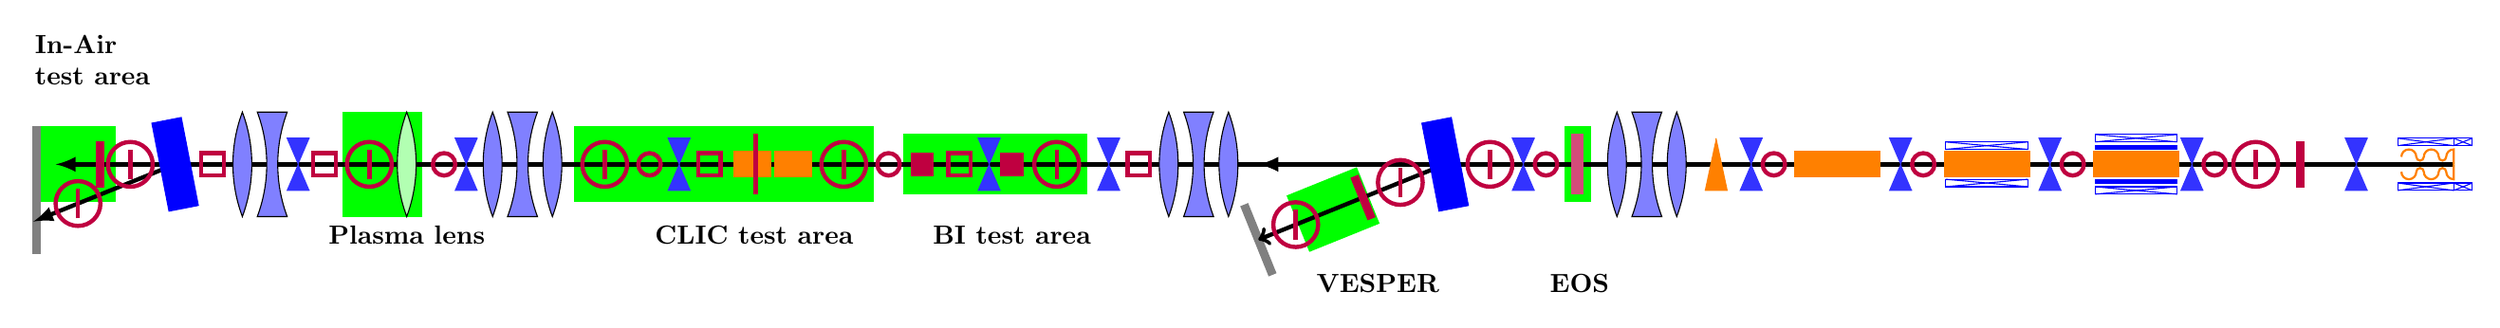
\begin{tikzpicture}
    \begin{scope}
      %% TIKZ DRAWING OF CALIFES ELEMENTS
%% TO BE INCLUDED INTO A LATEX DOCUMENT
%% INSIDE A TIKZPICTURE ENVIRONMENT
%% K. Sjobak, 2018--2020, D. Gamba 2020, L.A. Dyks 2021

    % Initialise some variables: %%%%%%%%%%%%%%%%%%%%%%%%%%%%%%%
    \pgfmathsetmacro{\VesperStart}{1.5}; %Center of the dipole (X)
    \pgfmathsetmacro{\VesperAngle}{-22.0};
    %Arrow end point
    \pgfmathsetmacro{\VesperX}{-1};
    \pgfmathsetmacro{\VesperY}{(\VesperStart-\VesperX)*tan(\VesperAngle)};

    \pgfmathsetmacro{\VesperTabX}{-0.0};
    \pgfmathsetmacro{\VesperTabY}{(\VesperStart-\VesperTabX)*tan(\VesperAngle)};

    \if\getvalue{distances}1
        \pgfmathsetmacro{\RFyOFF}{-0.0};
    \else
        \pgfmathsetmacro{\RFyOFF}{-0.5};
    \fi

    \if\getvalue{elemnames}1
        \pgfmathsetmacro{\BotLegyOFF}{0.0};
    \else
        \pgfmathsetmacro{\BotLegyOFF}{1.1};
    \fi
    %%%%%%%%%%%%%%%%%%%%%%%%%%%%%%%%%%%%%%%%%%%%%
    %% GREEN Area to indicate experiments
    %%%%%%%%%%%%%%%%%%%%%%%%%%%%%%%%%%%%%%%%%%%%%

    %EOS table
    \filldraw[green] (3.45, -0.5) rectangle (3.1,0.5);
    \node at (3.3, -2.7+\BotLegyOFF) {\textbf{EOS}};

    \filldraw[green,rotate around={-\VesperAngle:(\VesperTabX,\VesperTabY)}]
    (\VesperTabX-0.5, \VesperTabY-0.4) rectangle
    (\VesperTabX+0.5, \VesperTabY+0.4);
    %\node[rotate=-90,anchor=west] at (\VesperTabX,\VesperTabY-0.7) {\belemsiz VESPER};
    \node at (\VesperTabX+0.6, -2.7+\BotLegyOFF) {\textbf{VESPER}};

    %%%%%%%%%%%%%%%%%%%%%%%%%%%%%%%%%%%%%%%%%%%%%%%
    %%%%%%%%%%%%%%%%%%%%%%%%%%%%%%%%%%%%%%%%%%%%%%%
    %%%%%%%%%%%%%%%%%%%%%%%%%%%%%%%%%%%%%%%%%%%%%%%


    %% BEAM
    \if\getvalue{unbroken}0
        \draw[latex-,ultra thick] (0,0)--(15,0);
        \draw[ultra thick, dashed] (-1,0) -- (0,0);
    \else
        \draw[latex-,ultra thick] (-1,0)--(15,0);
    \fi

    %% GUN
    \if\getvalue{distances}1
        \node at (15,1) {\belemsiz 0.0~m};
    \fi

    % Gun solenoids
    \solRect{15}{0.25}{14.25}{0.35}
    \solRect{15}{-0.25}{14.25}{-0.35}

    \solRect{15.25}{0.25}{15}{0.35}
    \solRect{15.25}{-0.25}{15}{-0.35}

    % Gun cavity
    \draw[orange,  thick] (15,0.0) to (15,0.2)
        arc(90:180:0.1)
        arc(360:180:0.05) arc(0:180:0.1)
        arc(360:180:0.05) arc(0:180:0.1);
    \draw[orange, thick] (15,0.0) to (15,-0.2)
        arc(-90:-180:0.1)
        arc(0:180:0.05) arc(0:-180:0.1)
        arc(0:180:0.05) arc(0:-180:0.1);

    \if\getvalue{elemnames}1
        \node[rotate=-90,anchor=west,align=left] at (15+0.25/2, -0.7)
            {\belemsiz SNH 110};
        \node[rotate=-90,anchor=west,align=left] at (14.5, -0.7)
            {\belemsiz GUN 115\\
             \belemsiz SNI 120};
    \fi

    \correctorMagnet{13.7}{DG 130};
    \if\getvalue{distances}1
        \node at (13.7,1) {\belemsiz 0.32~m};
    \fi

    \if\getvalue{auxElems}1
        % Laser mirror
        \draw[ultra thick]  ({(13.7-13)/2+13 + 0.1}, -0.1) --
                        ({(13.7-13)/2+13 - 0.1}, -0.3);

        %Laser
        \draw[thick,-latex,dashed]
            ({(13.7-13)/2+13},-2.25+\BotLegyOFF) --
            ({(13.7-13)/2+13},-0.2) --
            (15,0);

        %Laser table
        \BTV[-2.25+\BotLegyOFF]{14}{};
        \draw[thick, -latex, dashed]
            (13,-2.25+\BotLegyOFF) -- (14,-2.25+\BotLegyOFF);
        \if\getvalue{elemnames}1
            \node at (14.9,-2.25) {\belemsiz BTV125};
        \fi

        \draw[ultra thick] ({(13.7-13)/2+13-0.25/2}, -2.25-0.25/2+\BotLegyOFF) --
                           ({(13.7-13)/2+13+0.25/2}, -2.25+0.25/2+\BotLegyOFF);
    \fi

    %ICT 210
    \filldraw[purple] (12.95-0.1/2,-0.3) rectangle (12.95+0.1/2,0.3);
    \if\getvalue{elemnames}1
        \node[rotate=-90,anchor=west] at (12.95,-0.7) {\belemsiz ICT 210};
    \fi

    \BTV{12.35}{MTV 215};
    \if\getvalue{distances}1
        \node at (12.35,0.6) {\belemsiz 1.81~m};
    \fi

    \cBPM{11.8}{BPC 220}{0.15};
    \correctorMagnet{11.5}{DG 225}; 
    %\node at (11.5,1) {\belemsiz 2.18~m}; !Moved to the bottom, to be drawn on top of RF network

    %ACS 230
    \filldraw[ultra thick, orange] (11.3,-0.15) rectangle (10.2,0.15);

    \solRect{11.3}{0.3}{10.2}{0.4}
    \solRect{11.3}{-0.3}{10.2}{-0.4}

    \filldraw[blue] (11.3, 0.2) rectangle (10.2,  0.25);
    \filldraw[blue] (11.3,-0.2) rectangle (10.2, -0.25);

    \if\getvalue{elemnames}1
        \node[rotate=-90,anchor=west, align=left] at (10.2+1.1/2,-0.7)
            {\belemsiz ACS 230\\
             \belemsiz DB 230-S\\
             \belemsiz SNG 230};
    \fi

    \cBPM{9.9}{BPC 240}{0.15};
    \correctorMagnet{9.6}{DG 245};
    %\node at (9.6,1) {\belemsiz 7.33~m}; !Moved to bottom

    % ACS 250
    \filldraw[ultra thick, orange] (9.3,-0.15) rectangle (8.2,0.15);
    \if\getvalue{elemnames}1
        \node[rotate=-90,anchor=west, align=left] at (8.2+1.1/2,-0.7) {\belemsiz ACS 250\\
                                                                       \belemsiz SNG 250};
    \fi

    \solRect{9.3}{0.2}{8.2}{0.3};
    \solRect{9.3}{-0.2}{8.2}{-0.3};

    \cBPM{7.9}{BPC 260}{0.15};
    \correctorMagnet{7.6}{DG 265};
    %\node at (7.6,1) {\belemsiz 12.49~m}; !Moved to bottom

    % ACS 270
    \filldraw[ultra thick, orange] (7.3,-0.15) rectangle (6.2,0.15);
    \if\getvalue{elemnames}1
        \node[rotate=-90,anchor=west] at (6.2+1.1/2,-0.7) {\belemsiz ACS 270};
    \fi

    %\node at (10,-2.25) {\textbf{CALIFES S-band injector}};

    \cBPM{5.9}{BPC 310}{0.15};
    \correctorMagnet{5.6}{DG 320};
    \if\getvalue{distances}1
        \node at (5.6,1) {\belemsiz 17.70~m};
    \fi

    \kickerHV[0]{5.125}{SDH 340}{-1}{orange};

    %\draw[ultra thick, purple] (4.15,-0.15) rectangle (3.85,0.15);

    \lensF{4.6}{QFD 350};
    \lensD{4.2}{QDD 355};
    \lensF{3.8}{QFD 360};
    %\node at (3.9,1) {\belemsiz 18.90~m};
    % unknown position after EOS installation
    \if\getvalue{distances}1
        \node at (4.1,1) {\belemsiz $\approx$19~m};
    \fi

    %%EOS table defined on top, to get behind the "beam"
    %\draw[-latex, dashed,thick] (4.8,-2) -- (4.8,-0.2) -- (3.0,-0.2) -- (3,-2);
    %%\node at (4.8,-2.25) {\belemsiz EOS laser};
    %\node at (3.9,-2.25) {\textbf{Electro-Optical Sampling}};
    \filldraw[purple!70] (3.2,-0.4) rectangle (3.35,0.4);
    \if\getvalue{elemnames}1
        \node[rotate=-90,anchor=west,align=left] at (3.275,-0.7)
            {\belemsiz EOS};
    \fi

    \cBPM{2.85}{BPC 380}{0.15};
    \correctorMagnet{2.55}{DG 385};
    %\node at (2.4,1) {\belemsiz 19.96~m};
    % unknown position after EOS installation
    \if\getvalue{distances}1
        \node at (2.55,1) {\belemsiz $\approx$20~m};
    \fi

    \BTV{2.1}{MTV 390};

    %% VESPER


    \filldraw[gray,rotate around={-\VesperAngle:(\VesperX,\VesperY)}]
        (\VesperX-0.05, \VesperY-0.5) rectangle
        (\VesperX+0.05, \VesperY+0.5);

    \draw[->,ultra thick] (\VesperStart,0)--(\VesperX,\VesperY);

    %\kickerHV[0]{\VesperStart}{BHB 400}{1}{blue};
    \dipole[0]{\VesperStart}{BHB 400}{{-\VesperAngle/2}};

    \pgfmathsetmacro{\VesperBTVaX}{0.9};
    \pgfmathsetmacro{\VesperBTVaY}{(\VesperStart-\VesperBTVaX)*tan(\VesperAngle)};
    \BTV[\VesperBTVaY]{\VesperBTVaX}{BTV420}

    % ICT 430
    \pgfmathsetmacro{\VesperICTX}{0.4};
    \pgfmathsetmacro{\VesperICTY}{(\VesperStart-\VesperICTX)*tan(\VesperAngle)};
    \filldraw[purple,rotate around={-\VesperAngle:(\VesperICTX,\VesperICTY)}]
        (\VesperICTX-0.1/2, \VesperICTY-0.3) rectangle
        (\VesperICTX+0.1/2, \VesperICTY+0.3);

    \if\getvalue{elemnames}1
        \node[rotate=-90,anchor=west] at (\VesperICTX,\VesperICTY-0.7) {\belemsiz ICT 430};
    \fi

    \pgfmathsetmacro{\VesperBTVbX}{-0.5};
    \pgfmathsetmacro{\VesperBTVbY}{(\VesperStart-\VesperBTVbX)*tan(\VesperAngle)};
    \BTV[\VesperBTVbY]{\VesperBTVbX}{BTV440}

    %% RF SYSTEM %%
    \if\getvalue{auxElems}1
        % MKS15
        \filldraw[orange!65] (12.35,1.0+\RFyOFF) -- (12.35+0.5,2+\RFyOFF) -- (12.35-0.5,2+\RFyOFF) -- cycle;
        \draw[-latex,orange!65,ultra thick] (12.35,1.75+\RFyOFF) -- (11.3,1.75+\RFyOFF) -- (11.3,0.4);

        \filldraw[orange!50] (11.6,1.75+\RFyOFF) circle (0.25);
        \if\getvalue{elemnames}1
            \node at (11.6,1.75+\RFyOFF) {\belemsiz $\Delta \Phi$};
        \fi

        \draw[-latex,orange!65,ultra thick] (12.35,1.75+\RFyOFF) -- (14.5+0.15/2,1.75+\RFyOFF) -- (14.5+0.15/2,0.4);

        \filldraw[orange!50] (14,1.75+\RFyOFF) circle (0.25);
        \if\getvalue{elemnames}1
            \node at (14,1.75+\RFyOFF) {\belemsiz $\Delta \Phi$};
        \fi

        \filldraw[orange!50] (13.25,1.75+\RFyOFF) circle (0.25);
        \if\getvalue{elemnames}1
            \node at (13.25,1.75+\RFyOFF) {\belemsiz $\Delta P$};
        \fi

        \if\getvalue{elemnames}1
            \node[align=center,anchor=north] at (12.35,2+\RFyOFF) {\belemsiz MKS\\ \belemsiz 15};
        \fi

        % MKS11
        \filldraw[orange!65] (10.7,1.0+\RFyOFF) -- (10.7+0.5,2+\RFyOFF) -- (10.7-0.5,2+\RFyOFF) -- cycle;
        \draw[orange!65, ultra thick, -latex] (10.5,1.75+\RFyOFF) -- (9.3,1.75+\RFyOFF) -- (9.3,0.3);
        \draw[orange!65, ultra thick, -latex] (10.5,1.75+\RFyOFF) -- (7.3,1.75+\RFyOFF) -- (7.3,0.2);

        \if\getvalue{elemnames}1
            \node[align=center,anchor=north] at (10.7,2+\RFyOFF) {\belemsiz MKS\\ \belemsiz 11};
        \fi

        % MKS31
        \filldraw[orange!65] (6.4,1.0+\RFyOFF) -- (6.4+0.5,2+\RFyOFF) -- (6.4-0.5,2+\RFyOFF) -- cycle;
        \draw[orange!65, ultra thick, -latex] (6.4,1.75+\RFyOFF) -- (5.125,1.75+\RFyOFF) -- (5.125,0.35);
        % \draw[orange, ultra thick, -latex] (10.5,1.75) -- (7.3,1.75) -- (7.3,0.4);

        \if\getvalue{elemnames}1
            \node[align=center,anchor=north] at (6.4,2+\RFyOFF) {\belemsiz MKS\\ \belemsiz 31};
        \fi
    \fi

    % Text on top of the orange
    \if\getvalue{distances}1
        \node at (11.5,1) {\belemsiz 2.18~m};
        \node at (9.6,1) {\belemsiz 7.33~m};
        \node at (7.6,1) {\belemsiz 12.49~m};
    \fi

%%% Local Variables:
%%% mode: latex
%%% TeX-master: "../layout.tex"
%%% End:

    \end{scope}
    \begin{scope}[shift={(-16.8,0)}]
      %% TIKZ DRAWING OF CLEAR EXPERIMENTAL BEAMLINE 1 ELEMENTS
%% TO BE INCLUDED INTO A LATEX DOCUMENT
%% INSIDE A TIKZPICTURE ENVIRONMENT
%% K. Sjobak, 2018--2020, D. Gamba 2020
%% Updated L.A. Dyks - removed CLIC BPMs

    \if\getvalue{elemnames}1
        \pgfmathsetmacro{\BotLegyOFF}{0.0};
    \else
        \pgfmathsetmacro{\BotLegyOFF}{1.3};
    \fi

    %%%%%%%%%%%%%%%%%%%%%%%%%%%%%%%%%%%%%%%%%%%%%
    %% GREEN Areas to indicate experiments
    %%%%%%%%%%%%%%%%%%%%%%%%%%%%%%%%%%%%%%%%%%%%%

    %BEAM INSTRUMENTATION TEST STAND AREA
    \filldraw[green] (11.05,-0.4) rectangle (13.5,0.4);
    \node at ({(11.3+13.7)/2},-2.25+\BotLegyOFF) {\textbf{BI test area}};

    %CLIC test area
    \filldraw[green] (10.65,-0.5) rectangle (6.65,0.5);
    \node at ({(10.3+7.8)/2},-2.25+\BotLegyOFF) {\textbf{CLIC test area}};

    %IN-AIR table
    \filldraw[green] (-0.6,-0.5) rectangle (0.5,0.5);
    \node[align=left,anchor=west] at (-0.7,1.4) {\textbf{In-Air}\\ \textbf{test area}};

    % PLASMA LENS
    \filldraw[green] (3.55,-0.7) rectangle (4.6,0.7);
    \node at (4.4,-2.25+\BotLegyOFF) {\textbf{Plasma lens}};

    %%%%%%%%%%%%%%%%%%%%%%%%%%%%%%%%%%%%%%%%%%%%%%%
    %%%%%%%%%%%%%%%%%%%%%%%%%%%%%%%%%%%%%%%%%%%%%%%
    %%%%%%%%%%%%%%%%%%%%%%%%%%%%%%%%%%%%%%%%%%%%%%%

    % FINAL DUMP
    \if\getvalue{elemnames}1
        \filldraw[gray] (-0.6,-2.0) rectangle (-0.5,0.5);
    \else
        \filldraw[gray] (-0.6,-1.2) rectangle (-0.5,0.5);
    \fi

    %THE BEAM
    \draw[latex-,ultra thick] (-0.3,0)--(16,0);

    % \kickerHV[0]{15.8}{BHB 400}{1}{blue};
    \if\getvalue{unbroken}0
        \dipole[0]{15.8}{BHB 400}{{10}};
    \fi


    \lensF{15.4}{QFD 510};
    \lensD{15.0}{QDD 515};
    \lensF{14.6}{QFD 520};
    \if\getvalue{distances}1
        \node at (15.0,1) {\belemsiz 22.86~m};
    \fi

    \iBPM{14.2}{BPM 530};

    \correctorMagnet{13.8}{DJ 540};
    \if\getvalue{distances}1
        \node at (13.8,1) {\belemsiz 23.98~m};
    \fi

    \BTV{13.1}{BTV 545};

    \filldraw[purple] (12.5+0.15,0.15) rectangle (12.5-0.15,-0.15);
    \if\getvalue{elemnames}1
        \node[rotate=-90,anchor=west] at (12.5,-0.7)
            {\belemsiz WCM 550};
    \fi

    \correctorMagnet{12.2}{DJ 590};
    \if\getvalue{distances}1
        \node at (12.4,1) {\belemsiz 25.21~m};
    \fi

    \iBPM{11.8} {BPM 595}; %{BPM 560};

    \filldraw[purple] (11.3+0.15,0.15) rectangle (11.3-0.15,-0.15);
    \if\getvalue{elemnames}1
        \node[rotate=-90,anchor=west] at (11.3,-0.7)
            {\belemsiz BPR 600};
    \fi

    %\cBPM{11.1}{BPC 565}{0.15};
    \cBPM{10.85}{BPC 610}{0.15};

    \BTV{10.25}{BTV 620};
    \if\getvalue{distances}1
        \node at (10.5,1) {\belemsiz 26.04~m};
    \fi

    \filldraw[ultra thick, orange] (9.80,-0.15) rectangle (9.35,0.15);
    \if\getvalue{elemnames}1
        \node[rotate=-90,anchor=west] at (9.45,-0.7)
            {\belemsiz ACS 640};
    \fi

    \filldraw[ultra thick, orange] (9.25,-0.15) rectangle (8.80,0.15);
    \filldraw[purple] (9.1,-0.4) rectangle (9.05,0.4);
    \if\getvalue{elemnames}1
        \node[rotate=-90,anchor=west,align=left] at (8.95,-0.7)
            {\belemsiz WFM 645\\[-0.3em]
             \belemsiz ACS 650};
    \fi

    %\cBPM{9.0}{BPC 660}{0.1};
    %\cBPM{8.7}{BPC 670}{0.1};
    %\cBPM{8.4}{BPC 680}{0.1};
    %\cBPM{8.1}{BPC 690}{0.1};

    \iBPM{8.45}{BPM 690};

    \correctorMagnet{8.05}{DJ 710};
    \if\getvalue{distances}1
        \node at (8.0,0.9) {\belemsiz 29.31~m};
    \fi
    

    \cBPM{7.65}{BPC 720}{0.15};

    \BTV{7.05}{BTV 730};
    \if\getvalue{distances}1
        \node at (7.15,0.65) {\belemsiz 29.75~m};
    \fi

    \lensF{6.35}{QFD 760};
    \lensD{5.95}{QDD 765};
    \lensF{5.55}{QFD 770};
    \if\getvalue{distances}1
        \node at (5.95,0.9) {\belemsiz 30.62~m};
    \fi


    \correctorMagnet{5.2}{DJ 780};
    \if\getvalue{distances}1
        \node at (5.2,1.15) {\belemsiz 31.66~m};
    \fi

    \cBPM{4.9}{BPC 790}{0.15};

    \lensF[green!30]{4.4}{PLC 800\\[-0.5em]
             \belemsiz BTV 800\\[-0.5em]
             \belemsiz BTV 805};
    \if\getvalue{distances}1
        \node at (4.4,0.9) {\belemsiz 32.26~m};
    \fi

    \BTV{3.9}{BTV 810};
    \if\getvalue{distances}1
        \node at (3.9,1.15) {\belemsiz 32.53~m};
    \fi

    \iBPM{3.3}{BPM 820};

    \correctorMagnet{2.95}{DJ 840};
    \if\getvalue{distances}1
        \node at (2.95,0.9) {\belemsiz 33.38~m};
    \fi

    \lensD{2.60}{QDD 870};
    \if\getvalue{distances}1
        \node at (2.35,1.15) {\belemsiz 33.92~m};
    \fi
    \lensF{2.2}{QFD 880};
    
    \iBPM{1.8}{BPM 890};
    %% IN-AIR SPECTROMETER

    \pgfmathsetmacro{\InAirStart}{1.3};
    \pgfmathsetmacro{\InAirAngle}{-22.0};
    \pgfmathsetmacro{\InAirY}{(\InAirStart+0.6)*tan(\InAirAngle)};

    \draw[-latex,ultra thick] (\InAirStart,0)--(-0.6,\InAirY);

    %\kickerHV[0]{\InAirStart}{BHB 900}{1}{blue};
    \dipole[0]{\InAirStart}{BHB 900}{{-\InAirAngle/2}};

    \if\getvalue{distances}1
        \node at (\InAirStart,0.9) {\belemsiz 35.03~m};
    \fi

    \pgfmathsetmacro{\InAirBTVaX}{0.0};
    \pgfmathsetmacro{\InAirBTVaY}{(\InAirStart-\InAirBTVaX)*tan(\InAirAngle)};
    \BTV[\InAirBTVaY]{\InAirBTVaX}{BTV930};

    %\pgfmathsetmacro{\InAirBPMx}{0.5};
    %\pgfmathsetmacro{\InAirBPMy}{(\InAirStart-\InAirBPMx)*tan(\InAirAngle)};
    %\iBPM[\InAirBPMy]{\InAirBPMx}{BPM920};

    %% IN-AIR TABLE INSTRUMENTATION
    \BTV{0.7}{BTV 910};
%    \node[anchor=south] at (0.9,0.3) {\belemsiz BTV 910};

    %ICT 210
    \filldraw[purple] (0.3-0.1/2,-0.3) rectangle (0.3+0.1/2,0.3);
    \if\getvalue{elemnames}1
        \node[anchor=south] at (0.3,0.45) {\belemsiz ICT 915};
    \fi

    %% RF SYSTEM
    \if\getvalue{auxElems}1
        \filldraw[orange!65] (11.2,0.7) -- (11.2+0.5,1.7) -- (11.2-0.5,1.7) -- cycle;
        \draw[ultra thick, orange!65,] (11.15,1.45) -- (9.25,1.45);
        \draw[ultra thick, orange!65, dashed, -latex] (9.25,1.45) -- (9.25,0.2);
        \draw[ultra thick, orange!65, dashed, -latex] (9.25,1.45) -- (9.25,0.8) -- (9.8,0.8) -- (9.8,0.2);
        \if\getvalue{elemnames}1
            \node[align=center,anchor=north] at (11.2,1.7) {\belemsiz MKX\\ \belemsiz 1};
        \fi
    \fi


%%% Local Variables:
%%% mode: latex
%%% TeX-master: "../layout.tex"
%%% End:

    \end{scope}
  \end{tikzpicture}
  % %% TIKZ DRAWING OF CALIFES ELEMENTS
%% TO BE INCLUDED INTO A LATEX DOCUMENT
%% K. Sjobak, 2018
%% L.A. Dyks 2021 - changed element colour boxes

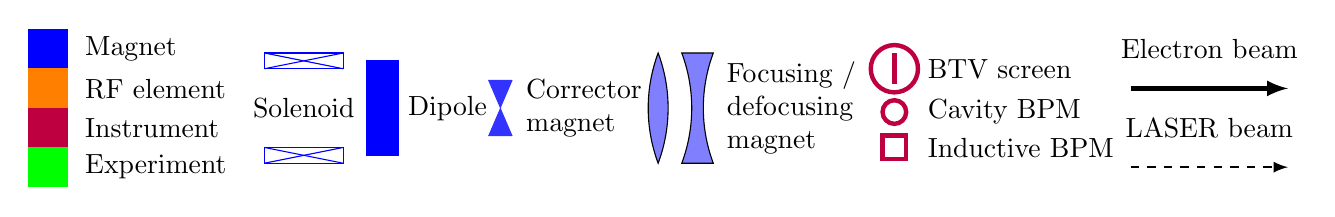
\begin{tikzpicture}
    
    \filldraw[blue] (-6.0,1.) rectangle (-5.5,0.5);
    \node[align=left,anchor=west] at (-5.4,0.75) {Magnet};

    \filldraw[orange] (-6.0,0.0) rectangle (-5.5,0.5);
    \node[align=left,anchor=west] at (-5.4,0.25) {RF element};
    
    \filldraw[purple] (-6.0,0.0) rectangle (-5.5,-0.5);
    \node[align=left,anchor=west] at (-5.4,-0.25) {Instrument};

    \filldraw[green] (-6.0,-0.5) rectangle (-5.5,-1.);
    \node[align=left,anchor=west] at (-5.4,-0.75) {Experiment};
    
    \solRect{-3.0}{0.5}{-2.0}{0.7};
    \solRect{-3.0}{-0.5}{-2.0}{-0.7};
    %\draw[->,ultra thick] (-3.2,0)--(-3.8,0);
    \node at (-2.5,0) {Solenoid};

    %\kickerHV[0]{-1.5}{}{1}{blue};
    \dipole[0]{-1.5}{}{0};
    \node[align=left,anchor=west] at (-1.3,0) {Dipole};

    \correctorMagnet{0.0}{};
    \node[align=left,anchor=west] at (0.2,0) {Corrector\\ magnet};
    
    \lensF{2.0}{};
    \lensD{2.5}{};
    \node[align=left,anchor=west] at (2.75,0) {Focusing /\\ defocusing\\ magnet};

    \BTV[0.5]{5}{};
    \node[align=left,anchor=west] at (5.3,0.5) {BTV screen};
    
    \cBPM[-0.05]{5}{}{0.15};
    \node[align=left,anchor=west] at (5.3,-0.05) {Cavity BPM};
    
    \iBPM[-0.5]{5}{};
    \node[align=left,anchor=west] at (5.3,-0.5) {Inductive BPM};

    \node at (9,0.75) {Electron beam};
    \draw[ultra thick, -latex] (8,0.25) -- (10,0.25);

    \node at (9,-0.25) {LASER beam};
    \draw[thick, dashed, -latex] (8,-0.75) -- (10,-0.75);

\end{tikzpicture}

\end{center}
\noindent\makebox[\linewidth]{\rule{\linewidth}{1.0pt}}

%\newpage
\subsection{Simplified (no distances or element names)}
\begin{center}
  \setvalue{distances = 0}
  \setvalue{elemnames = 0}
  \setvalue{auxElems  = 1}
  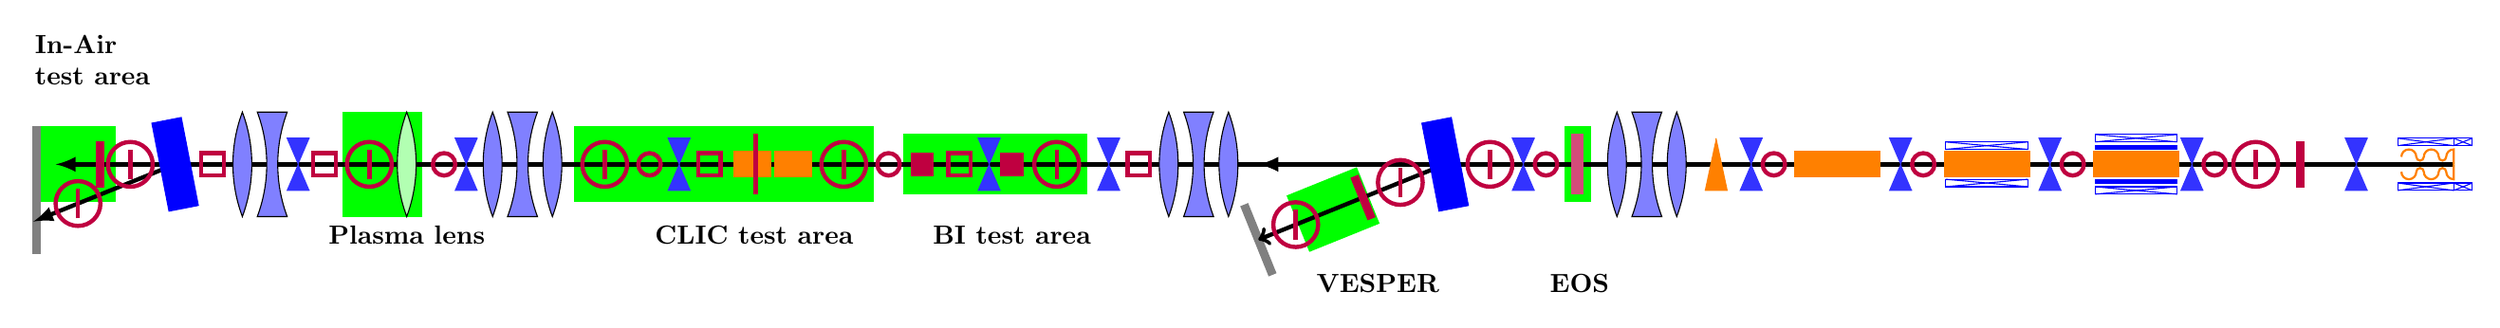
\begin{tikzpicture}
    \begin{scope}
      %% TIKZ DRAWING OF CALIFES ELEMENTS
%% TO BE INCLUDED INTO A LATEX DOCUMENT
%% INSIDE A TIKZPICTURE ENVIRONMENT
%% K. Sjobak, 2018--2020, D. Gamba 2020, L.A. Dyks 2021

    % Initialise some variables: %%%%%%%%%%%%%%%%%%%%%%%%%%%%%%%
    \pgfmathsetmacro{\VesperStart}{1.5}; %Center of the dipole (X)
    \pgfmathsetmacro{\VesperAngle}{-22.0};
    %Arrow end point
    \pgfmathsetmacro{\VesperX}{-1};
    \pgfmathsetmacro{\VesperY}{(\VesperStart-\VesperX)*tan(\VesperAngle)};

    \pgfmathsetmacro{\VesperTabX}{-0.0};
    \pgfmathsetmacro{\VesperTabY}{(\VesperStart-\VesperTabX)*tan(\VesperAngle)};

    \if\getvalue{distances}1
        \pgfmathsetmacro{\RFyOFF}{-0.0};
    \else
        \pgfmathsetmacro{\RFyOFF}{-0.5};
    \fi

    \if\getvalue{elemnames}1
        \pgfmathsetmacro{\BotLegyOFF}{0.0};
    \else
        \pgfmathsetmacro{\BotLegyOFF}{1.1};
    \fi
    %%%%%%%%%%%%%%%%%%%%%%%%%%%%%%%%%%%%%%%%%%%%%
    %% GREEN Area to indicate experiments
    %%%%%%%%%%%%%%%%%%%%%%%%%%%%%%%%%%%%%%%%%%%%%

    %EOS table
    \filldraw[green] (3.45, -0.5) rectangle (3.1,0.5);
    \node at (3.3, -2.7+\BotLegyOFF) {\textbf{EOS}};

    \filldraw[green,rotate around={-\VesperAngle:(\VesperTabX,\VesperTabY)}]
    (\VesperTabX-0.5, \VesperTabY-0.4) rectangle
    (\VesperTabX+0.5, \VesperTabY+0.4);
    %\node[rotate=-90,anchor=west] at (\VesperTabX,\VesperTabY-0.7) {\belemsiz VESPER};
    \node at (\VesperTabX+0.6, -2.7+\BotLegyOFF) {\textbf{VESPER}};

    %%%%%%%%%%%%%%%%%%%%%%%%%%%%%%%%%%%%%%%%%%%%%%%
    %%%%%%%%%%%%%%%%%%%%%%%%%%%%%%%%%%%%%%%%%%%%%%%
    %%%%%%%%%%%%%%%%%%%%%%%%%%%%%%%%%%%%%%%%%%%%%%%


    %% BEAM
    \if\getvalue{unbroken}0
        \draw[latex-,ultra thick] (0,0)--(15,0);
        \draw[ultra thick, dashed] (-1,0) -- (0,0);
    \else
        \draw[latex-,ultra thick] (-1,0)--(15,0);
    \fi

    %% GUN
    \if\getvalue{distances}1
        \node at (15,1) {\belemsiz 0.0~m};
    \fi

    % Gun solenoids
    \solRect{15}{0.25}{14.25}{0.35}
    \solRect{15}{-0.25}{14.25}{-0.35}

    \solRect{15.25}{0.25}{15}{0.35}
    \solRect{15.25}{-0.25}{15}{-0.35}

    % Gun cavity
    \draw[orange,  thick] (15,0.0) to (15,0.2)
        arc(90:180:0.1)
        arc(360:180:0.05) arc(0:180:0.1)
        arc(360:180:0.05) arc(0:180:0.1);
    \draw[orange, thick] (15,0.0) to (15,-0.2)
        arc(-90:-180:0.1)
        arc(0:180:0.05) arc(0:-180:0.1)
        arc(0:180:0.05) arc(0:-180:0.1);

    \if\getvalue{elemnames}1
        \node[rotate=-90,anchor=west,align=left] at (15+0.25/2, -0.7)
            {\belemsiz SNH 110};
        \node[rotate=-90,anchor=west,align=left] at (14.5, -0.7)
            {\belemsiz GUN 115\\
             \belemsiz SNI 120};
    \fi

    \correctorMagnet{13.7}{DG 130};
    \if\getvalue{distances}1
        \node at (13.7,1) {\belemsiz 0.32~m};
    \fi

    \if\getvalue{auxElems}1
        % Laser mirror
        \draw[ultra thick]  ({(13.7-13)/2+13 + 0.1}, -0.1) --
                        ({(13.7-13)/2+13 - 0.1}, -0.3);

        %Laser
        \draw[thick,-latex,dashed]
            ({(13.7-13)/2+13},-2.25+\BotLegyOFF) --
            ({(13.7-13)/2+13},-0.2) --
            (15,0);

        %Laser table
        \BTV[-2.25+\BotLegyOFF]{14}{};
        \draw[thick, -latex, dashed]
            (13,-2.25+\BotLegyOFF) -- (14,-2.25+\BotLegyOFF);
        \if\getvalue{elemnames}1
            \node at (14.9,-2.25) {\belemsiz BTV125};
        \fi

        \draw[ultra thick] ({(13.7-13)/2+13-0.25/2}, -2.25-0.25/2+\BotLegyOFF) --
                           ({(13.7-13)/2+13+0.25/2}, -2.25+0.25/2+\BotLegyOFF);
    \fi

    %ICT 210
    \filldraw[purple] (12.95-0.1/2,-0.3) rectangle (12.95+0.1/2,0.3);
    \if\getvalue{elemnames}1
        \node[rotate=-90,anchor=west] at (12.95,-0.7) {\belemsiz ICT 210};
    \fi

    \BTV{12.35}{MTV 215};
    \if\getvalue{distances}1
        \node at (12.35,0.6) {\belemsiz 1.81~m};
    \fi

    \cBPM{11.8}{BPC 220}{0.15};
    \correctorMagnet{11.5}{DG 225}; 
    %\node at (11.5,1) {\belemsiz 2.18~m}; !Moved to the bottom, to be drawn on top of RF network

    %ACS 230
    \filldraw[ultra thick, orange] (11.3,-0.15) rectangle (10.2,0.15);

    \solRect{11.3}{0.3}{10.2}{0.4}
    \solRect{11.3}{-0.3}{10.2}{-0.4}

    \filldraw[blue] (11.3, 0.2) rectangle (10.2,  0.25);
    \filldraw[blue] (11.3,-0.2) rectangle (10.2, -0.25);

    \if\getvalue{elemnames}1
        \node[rotate=-90,anchor=west, align=left] at (10.2+1.1/2,-0.7)
            {\belemsiz ACS 230\\
             \belemsiz DB 230-S\\
             \belemsiz SNG 230};
    \fi

    \cBPM{9.9}{BPC 240}{0.15};
    \correctorMagnet{9.6}{DG 245};
    %\node at (9.6,1) {\belemsiz 7.33~m}; !Moved to bottom

    % ACS 250
    \filldraw[ultra thick, orange] (9.3,-0.15) rectangle (8.2,0.15);
    \if\getvalue{elemnames}1
        \node[rotate=-90,anchor=west, align=left] at (8.2+1.1/2,-0.7) {\belemsiz ACS 250\\
                                                                       \belemsiz SNG 250};
    \fi

    \solRect{9.3}{0.2}{8.2}{0.3};
    \solRect{9.3}{-0.2}{8.2}{-0.3};

    \cBPM{7.9}{BPC 260}{0.15};
    \correctorMagnet{7.6}{DG 265};
    %\node at (7.6,1) {\belemsiz 12.49~m}; !Moved to bottom

    % ACS 270
    \filldraw[ultra thick, orange] (7.3,-0.15) rectangle (6.2,0.15);
    \if\getvalue{elemnames}1
        \node[rotate=-90,anchor=west] at (6.2+1.1/2,-0.7) {\belemsiz ACS 270};
    \fi

    %\node at (10,-2.25) {\textbf{CALIFES S-band injector}};

    \cBPM{5.9}{BPC 310}{0.15};
    \correctorMagnet{5.6}{DG 320};
    \if\getvalue{distances}1
        \node at (5.6,1) {\belemsiz 17.70~m};
    \fi

    \kickerHV[0]{5.125}{SDH 340}{-1}{orange};

    %\draw[ultra thick, purple] (4.15,-0.15) rectangle (3.85,0.15);

    \lensF{4.6}{QFD 350};
    \lensD{4.2}{QDD 355};
    \lensF{3.8}{QFD 360};
    %\node at (3.9,1) {\belemsiz 18.90~m};
    % unknown position after EOS installation
    \if\getvalue{distances}1
        \node at (4.1,1) {\belemsiz $\approx$19~m};
    \fi

    %%EOS table defined on top, to get behind the "beam"
    %\draw[-latex, dashed,thick] (4.8,-2) -- (4.8,-0.2) -- (3.0,-0.2) -- (3,-2);
    %%\node at (4.8,-2.25) {\belemsiz EOS laser};
    %\node at (3.9,-2.25) {\textbf{Electro-Optical Sampling}};
    \filldraw[purple!70] (3.2,-0.4) rectangle (3.35,0.4);
    \if\getvalue{elemnames}1
        \node[rotate=-90,anchor=west,align=left] at (3.275,-0.7)
            {\belemsiz EOS};
    \fi

    \cBPM{2.85}{BPC 380}{0.15};
    \correctorMagnet{2.55}{DG 385};
    %\node at (2.4,1) {\belemsiz 19.96~m};
    % unknown position after EOS installation
    \if\getvalue{distances}1
        \node at (2.55,1) {\belemsiz $\approx$20~m};
    \fi

    \BTV{2.1}{MTV 390};

    %% VESPER


    \filldraw[gray,rotate around={-\VesperAngle:(\VesperX,\VesperY)}]
        (\VesperX-0.05, \VesperY-0.5) rectangle
        (\VesperX+0.05, \VesperY+0.5);

    \draw[->,ultra thick] (\VesperStart,0)--(\VesperX,\VesperY);

    %\kickerHV[0]{\VesperStart}{BHB 400}{1}{blue};
    \dipole[0]{\VesperStart}{BHB 400}{{-\VesperAngle/2}};

    \pgfmathsetmacro{\VesperBTVaX}{0.9};
    \pgfmathsetmacro{\VesperBTVaY}{(\VesperStart-\VesperBTVaX)*tan(\VesperAngle)};
    \BTV[\VesperBTVaY]{\VesperBTVaX}{BTV420}

    % ICT 430
    \pgfmathsetmacro{\VesperICTX}{0.4};
    \pgfmathsetmacro{\VesperICTY}{(\VesperStart-\VesperICTX)*tan(\VesperAngle)};
    \filldraw[purple,rotate around={-\VesperAngle:(\VesperICTX,\VesperICTY)}]
        (\VesperICTX-0.1/2, \VesperICTY-0.3) rectangle
        (\VesperICTX+0.1/2, \VesperICTY+0.3);

    \if\getvalue{elemnames}1
        \node[rotate=-90,anchor=west] at (\VesperICTX,\VesperICTY-0.7) {\belemsiz ICT 430};
    \fi

    \pgfmathsetmacro{\VesperBTVbX}{-0.5};
    \pgfmathsetmacro{\VesperBTVbY}{(\VesperStart-\VesperBTVbX)*tan(\VesperAngle)};
    \BTV[\VesperBTVbY]{\VesperBTVbX}{BTV440}

    %% RF SYSTEM %%
    \if\getvalue{auxElems}1
        % MKS15
        \filldraw[orange!65] (12.35,1.0+\RFyOFF) -- (12.35+0.5,2+\RFyOFF) -- (12.35-0.5,2+\RFyOFF) -- cycle;
        \draw[-latex,orange!65,ultra thick] (12.35,1.75+\RFyOFF) -- (11.3,1.75+\RFyOFF) -- (11.3,0.4);

        \filldraw[orange!50] (11.6,1.75+\RFyOFF) circle (0.25);
        \if\getvalue{elemnames}1
            \node at (11.6,1.75+\RFyOFF) {\belemsiz $\Delta \Phi$};
        \fi

        \draw[-latex,orange!65,ultra thick] (12.35,1.75+\RFyOFF) -- (14.5+0.15/2,1.75+\RFyOFF) -- (14.5+0.15/2,0.4);

        \filldraw[orange!50] (14,1.75+\RFyOFF) circle (0.25);
        \if\getvalue{elemnames}1
            \node at (14,1.75+\RFyOFF) {\belemsiz $\Delta \Phi$};
        \fi

        \filldraw[orange!50] (13.25,1.75+\RFyOFF) circle (0.25);
        \if\getvalue{elemnames}1
            \node at (13.25,1.75+\RFyOFF) {\belemsiz $\Delta P$};
        \fi

        \if\getvalue{elemnames}1
            \node[align=center,anchor=north] at (12.35,2+\RFyOFF) {\belemsiz MKS\\ \belemsiz 15};
        \fi

        % MKS11
        \filldraw[orange!65] (10.7,1.0+\RFyOFF) -- (10.7+0.5,2+\RFyOFF) -- (10.7-0.5,2+\RFyOFF) -- cycle;
        \draw[orange!65, ultra thick, -latex] (10.5,1.75+\RFyOFF) -- (9.3,1.75+\RFyOFF) -- (9.3,0.3);
        \draw[orange!65, ultra thick, -latex] (10.5,1.75+\RFyOFF) -- (7.3,1.75+\RFyOFF) -- (7.3,0.2);

        \if\getvalue{elemnames}1
            \node[align=center,anchor=north] at (10.7,2+\RFyOFF) {\belemsiz MKS\\ \belemsiz 11};
        \fi

        % MKS31
        \filldraw[orange!65] (6.4,1.0+\RFyOFF) -- (6.4+0.5,2+\RFyOFF) -- (6.4-0.5,2+\RFyOFF) -- cycle;
        \draw[orange!65, ultra thick, -latex] (6.4,1.75+\RFyOFF) -- (5.125,1.75+\RFyOFF) -- (5.125,0.35);
        % \draw[orange, ultra thick, -latex] (10.5,1.75) -- (7.3,1.75) -- (7.3,0.4);

        \if\getvalue{elemnames}1
            \node[align=center,anchor=north] at (6.4,2+\RFyOFF) {\belemsiz MKS\\ \belemsiz 31};
        \fi
    \fi

    % Text on top of the orange
    \if\getvalue{distances}1
        \node at (11.5,1) {\belemsiz 2.18~m};
        \node at (9.6,1) {\belemsiz 7.33~m};
        \node at (7.6,1) {\belemsiz 12.49~m};
    \fi

%%% Local Variables:
%%% mode: latex
%%% TeX-master: "../layout.tex"
%%% End:

    \end{scope}
    \begin{scope}[shift={(-16.8,0)}]
      %% TIKZ DRAWING OF CLEAR EXPERIMENTAL BEAMLINE 1 ELEMENTS
%% TO BE INCLUDED INTO A LATEX DOCUMENT
%% INSIDE A TIKZPICTURE ENVIRONMENT
%% K. Sjobak, 2018--2020, D. Gamba 2020
%% Updated L.A. Dyks - removed CLIC BPMs

    \if\getvalue{elemnames}1
        \pgfmathsetmacro{\BotLegyOFF}{0.0};
    \else
        \pgfmathsetmacro{\BotLegyOFF}{1.3};
    \fi

    %%%%%%%%%%%%%%%%%%%%%%%%%%%%%%%%%%%%%%%%%%%%%
    %% GREEN Areas to indicate experiments
    %%%%%%%%%%%%%%%%%%%%%%%%%%%%%%%%%%%%%%%%%%%%%

    %BEAM INSTRUMENTATION TEST STAND AREA
    \filldraw[green] (11.05,-0.4) rectangle (13.5,0.4);
    \node at ({(11.3+13.7)/2},-2.25+\BotLegyOFF) {\textbf{BI test area}};

    %CLIC test area
    \filldraw[green] (10.65,-0.5) rectangle (6.65,0.5);
    \node at ({(10.3+7.8)/2},-2.25+\BotLegyOFF) {\textbf{CLIC test area}};

    %IN-AIR table
    \filldraw[green] (-0.6,-0.5) rectangle (0.5,0.5);
    \node[align=left,anchor=west] at (-0.7,1.4) {\textbf{In-Air}\\ \textbf{test area}};

    % PLASMA LENS
    \filldraw[green] (3.55,-0.7) rectangle (4.6,0.7);
    \node at (4.4,-2.25+\BotLegyOFF) {\textbf{Plasma lens}};

    %%%%%%%%%%%%%%%%%%%%%%%%%%%%%%%%%%%%%%%%%%%%%%%
    %%%%%%%%%%%%%%%%%%%%%%%%%%%%%%%%%%%%%%%%%%%%%%%
    %%%%%%%%%%%%%%%%%%%%%%%%%%%%%%%%%%%%%%%%%%%%%%%

    % FINAL DUMP
    \if\getvalue{elemnames}1
        \filldraw[gray] (-0.6,-2.0) rectangle (-0.5,0.5);
    \else
        \filldraw[gray] (-0.6,-1.2) rectangle (-0.5,0.5);
    \fi

    %THE BEAM
    \draw[latex-,ultra thick] (-0.3,0)--(16,0);

    % \kickerHV[0]{15.8}{BHB 400}{1}{blue};
    \if\getvalue{unbroken}0
        \dipole[0]{15.8}{BHB 400}{{10}};
    \fi


    \lensF{15.4}{QFD 510};
    \lensD{15.0}{QDD 515};
    \lensF{14.6}{QFD 520};
    \if\getvalue{distances}1
        \node at (15.0,1) {\belemsiz 22.86~m};
    \fi

    \iBPM{14.2}{BPM 530};

    \correctorMagnet{13.8}{DJ 540};
    \if\getvalue{distances}1
        \node at (13.8,1) {\belemsiz 23.98~m};
    \fi

    \BTV{13.1}{BTV 545};

    \filldraw[purple] (12.5+0.15,0.15) rectangle (12.5-0.15,-0.15);
    \if\getvalue{elemnames}1
        \node[rotate=-90,anchor=west] at (12.5,-0.7)
            {\belemsiz WCM 550};
    \fi

    \correctorMagnet{12.2}{DJ 590};
    \if\getvalue{distances}1
        \node at (12.4,1) {\belemsiz 25.21~m};
    \fi

    \iBPM{11.8} {BPM 595}; %{BPM 560};

    \filldraw[purple] (11.3+0.15,0.15) rectangle (11.3-0.15,-0.15);
    \if\getvalue{elemnames}1
        \node[rotate=-90,anchor=west] at (11.3,-0.7)
            {\belemsiz BPR 600};
    \fi

    %\cBPM{11.1}{BPC 565}{0.15};
    \cBPM{10.85}{BPC 610}{0.15};

    \BTV{10.25}{BTV 620};
    \if\getvalue{distances}1
        \node at (10.5,1) {\belemsiz 26.04~m};
    \fi

    \filldraw[ultra thick, orange] (9.80,-0.15) rectangle (9.35,0.15);
    \if\getvalue{elemnames}1
        \node[rotate=-90,anchor=west] at (9.45,-0.7)
            {\belemsiz ACS 640};
    \fi

    \filldraw[ultra thick, orange] (9.25,-0.15) rectangle (8.80,0.15);
    \filldraw[purple] (9.1,-0.4) rectangle (9.05,0.4);
    \if\getvalue{elemnames}1
        \node[rotate=-90,anchor=west,align=left] at (8.95,-0.7)
            {\belemsiz WFM 645\\[-0.3em]
             \belemsiz ACS 650};
    \fi

    %\cBPM{9.0}{BPC 660}{0.1};
    %\cBPM{8.7}{BPC 670}{0.1};
    %\cBPM{8.4}{BPC 680}{0.1};
    %\cBPM{8.1}{BPC 690}{0.1};

    \iBPM{8.45}{BPM 690};

    \correctorMagnet{8.05}{DJ 710};
    \if\getvalue{distances}1
        \node at (8.0,0.9) {\belemsiz 29.31~m};
    \fi
    

    \cBPM{7.65}{BPC 720}{0.15};

    \BTV{7.05}{BTV 730};
    \if\getvalue{distances}1
        \node at (7.15,0.65) {\belemsiz 29.75~m};
    \fi

    \lensF{6.35}{QFD 760};
    \lensD{5.95}{QDD 765};
    \lensF{5.55}{QFD 770};
    \if\getvalue{distances}1
        \node at (5.95,0.9) {\belemsiz 30.62~m};
    \fi


    \correctorMagnet{5.2}{DJ 780};
    \if\getvalue{distances}1
        \node at (5.2,1.15) {\belemsiz 31.66~m};
    \fi

    \cBPM{4.9}{BPC 790}{0.15};

    \lensF[green!30]{4.4}{PLC 800\\[-0.5em]
             \belemsiz BTV 800\\[-0.5em]
             \belemsiz BTV 805};
    \if\getvalue{distances}1
        \node at (4.4,0.9) {\belemsiz 32.26~m};
    \fi

    \BTV{3.9}{BTV 810};
    \if\getvalue{distances}1
        \node at (3.9,1.15) {\belemsiz 32.53~m};
    \fi

    \iBPM{3.3}{BPM 820};

    \correctorMagnet{2.95}{DJ 840};
    \if\getvalue{distances}1
        \node at (2.95,0.9) {\belemsiz 33.38~m};
    \fi

    \lensD{2.60}{QDD 870};
    \if\getvalue{distances}1
        \node at (2.35,1.15) {\belemsiz 33.92~m};
    \fi
    \lensF{2.2}{QFD 880};
    
    \iBPM{1.8}{BPM 890};
    %% IN-AIR SPECTROMETER

    \pgfmathsetmacro{\InAirStart}{1.3};
    \pgfmathsetmacro{\InAirAngle}{-22.0};
    \pgfmathsetmacro{\InAirY}{(\InAirStart+0.6)*tan(\InAirAngle)};

    \draw[-latex,ultra thick] (\InAirStart,0)--(-0.6,\InAirY);

    %\kickerHV[0]{\InAirStart}{BHB 900}{1}{blue};
    \dipole[0]{\InAirStart}{BHB 900}{{-\InAirAngle/2}};

    \if\getvalue{distances}1
        \node at (\InAirStart,0.9) {\belemsiz 35.03~m};
    \fi

    \pgfmathsetmacro{\InAirBTVaX}{0.0};
    \pgfmathsetmacro{\InAirBTVaY}{(\InAirStart-\InAirBTVaX)*tan(\InAirAngle)};
    \BTV[\InAirBTVaY]{\InAirBTVaX}{BTV930};

    %\pgfmathsetmacro{\InAirBPMx}{0.5};
    %\pgfmathsetmacro{\InAirBPMy}{(\InAirStart-\InAirBPMx)*tan(\InAirAngle)};
    %\iBPM[\InAirBPMy]{\InAirBPMx}{BPM920};

    %% IN-AIR TABLE INSTRUMENTATION
    \BTV{0.7}{BTV 910};
%    \node[anchor=south] at (0.9,0.3) {\belemsiz BTV 910};

    %ICT 210
    \filldraw[purple] (0.3-0.1/2,-0.3) rectangle (0.3+0.1/2,0.3);
    \if\getvalue{elemnames}1
        \node[anchor=south] at (0.3,0.45) {\belemsiz ICT 915};
    \fi

    %% RF SYSTEM
    \if\getvalue{auxElems}1
        \filldraw[orange!65] (11.2,0.7) -- (11.2+0.5,1.7) -- (11.2-0.5,1.7) -- cycle;
        \draw[ultra thick, orange!65,] (11.15,1.45) -- (9.25,1.45);
        \draw[ultra thick, orange!65, dashed, -latex] (9.25,1.45) -- (9.25,0.2);
        \draw[ultra thick, orange!65, dashed, -latex] (9.25,1.45) -- (9.25,0.8) -- (9.8,0.8) -- (9.8,0.2);
        \if\getvalue{elemnames}1
            \node[align=center,anchor=north] at (11.2,1.7) {\belemsiz MKX\\ \belemsiz 1};
        \fi
    \fi


%%% Local Variables:
%%% mode: latex
%%% TeX-master: "../layout.tex"
%%% End:

    \end{scope}
  \end{tikzpicture}
\end{center}
\noindent\makebox[\linewidth]{\rule{\linewidth}{1.0pt}}

%\newpage
\subsection{Beamline only (no distances, element names, RF, or laser)}
\begin{center}
  \setvalue{distances = 0}
  \setvalue{elemnames = 0}
  \setvalue{auxElems  = 0}
  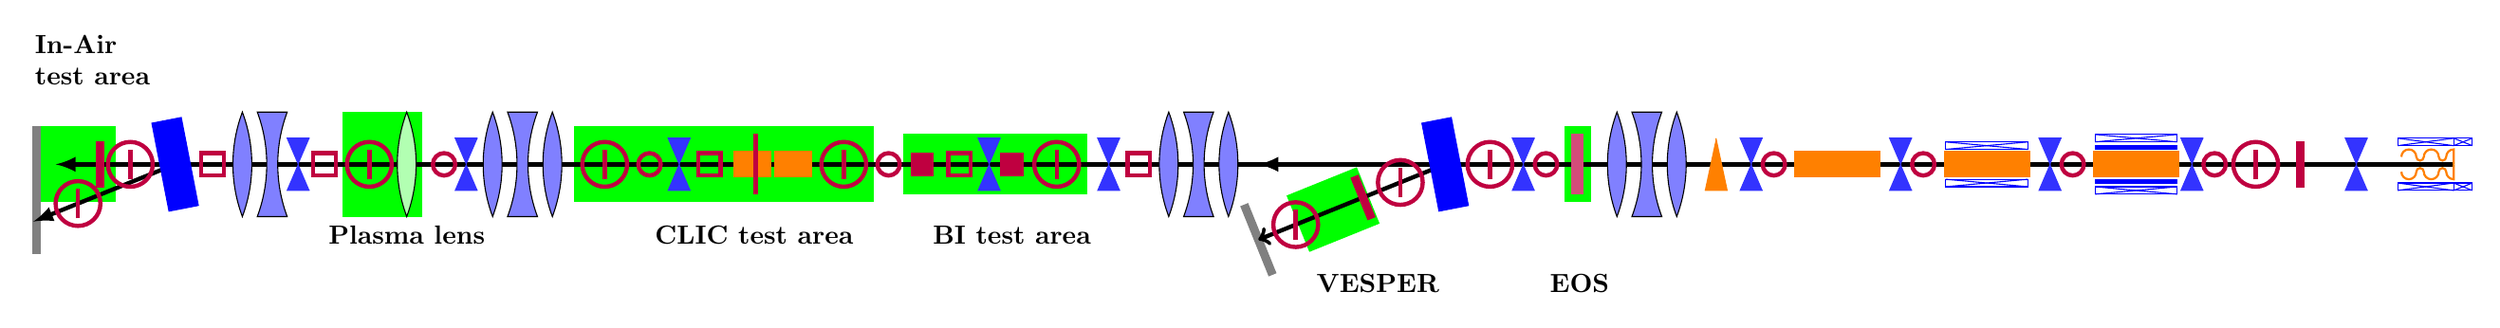
\begin{tikzpicture}
    \begin{scope}
      %% TIKZ DRAWING OF CALIFES ELEMENTS
%% TO BE INCLUDED INTO A LATEX DOCUMENT
%% INSIDE A TIKZPICTURE ENVIRONMENT
%% K. Sjobak, 2018--2020, D. Gamba 2020, L.A. Dyks 2021

    % Initialise some variables: %%%%%%%%%%%%%%%%%%%%%%%%%%%%%%%
    \pgfmathsetmacro{\VesperStart}{1.5}; %Center of the dipole (X)
    \pgfmathsetmacro{\VesperAngle}{-22.0};
    %Arrow end point
    \pgfmathsetmacro{\VesperX}{-1};
    \pgfmathsetmacro{\VesperY}{(\VesperStart-\VesperX)*tan(\VesperAngle)};

    \pgfmathsetmacro{\VesperTabX}{-0.0};
    \pgfmathsetmacro{\VesperTabY}{(\VesperStart-\VesperTabX)*tan(\VesperAngle)};

    \if\getvalue{distances}1
        \pgfmathsetmacro{\RFyOFF}{-0.0};
    \else
        \pgfmathsetmacro{\RFyOFF}{-0.5};
    \fi

    \if\getvalue{elemnames}1
        \pgfmathsetmacro{\BotLegyOFF}{0.0};
    \else
        \pgfmathsetmacro{\BotLegyOFF}{1.1};
    \fi
    %%%%%%%%%%%%%%%%%%%%%%%%%%%%%%%%%%%%%%%%%%%%%
    %% GREEN Area to indicate experiments
    %%%%%%%%%%%%%%%%%%%%%%%%%%%%%%%%%%%%%%%%%%%%%

    %EOS table
    \filldraw[green] (3.45, -0.5) rectangle (3.1,0.5);
    \node at (3.3, -2.7+\BotLegyOFF) {\textbf{EOS}};

    \filldraw[green,rotate around={-\VesperAngle:(\VesperTabX,\VesperTabY)}]
    (\VesperTabX-0.5, \VesperTabY-0.4) rectangle
    (\VesperTabX+0.5, \VesperTabY+0.4);
    %\node[rotate=-90,anchor=west] at (\VesperTabX,\VesperTabY-0.7) {\belemsiz VESPER};
    \node at (\VesperTabX+0.6, -2.7+\BotLegyOFF) {\textbf{VESPER}};

    %%%%%%%%%%%%%%%%%%%%%%%%%%%%%%%%%%%%%%%%%%%%%%%
    %%%%%%%%%%%%%%%%%%%%%%%%%%%%%%%%%%%%%%%%%%%%%%%
    %%%%%%%%%%%%%%%%%%%%%%%%%%%%%%%%%%%%%%%%%%%%%%%


    %% BEAM
    \if\getvalue{unbroken}0
        \draw[latex-,ultra thick] (0,0)--(15,0);
        \draw[ultra thick, dashed] (-1,0) -- (0,0);
    \else
        \draw[latex-,ultra thick] (-1,0)--(15,0);
    \fi

    %% GUN
    \if\getvalue{distances}1
        \node at (15,1) {\belemsiz 0.0~m};
    \fi

    % Gun solenoids
    \solRect{15}{0.25}{14.25}{0.35}
    \solRect{15}{-0.25}{14.25}{-0.35}

    \solRect{15.25}{0.25}{15}{0.35}
    \solRect{15.25}{-0.25}{15}{-0.35}

    % Gun cavity
    \draw[orange,  thick] (15,0.0) to (15,0.2)
        arc(90:180:0.1)
        arc(360:180:0.05) arc(0:180:0.1)
        arc(360:180:0.05) arc(0:180:0.1);
    \draw[orange, thick] (15,0.0) to (15,-0.2)
        arc(-90:-180:0.1)
        arc(0:180:0.05) arc(0:-180:0.1)
        arc(0:180:0.05) arc(0:-180:0.1);

    \if\getvalue{elemnames}1
        \node[rotate=-90,anchor=west,align=left] at (15+0.25/2, -0.7)
            {\belemsiz SNH 110};
        \node[rotate=-90,anchor=west,align=left] at (14.5, -0.7)
            {\belemsiz GUN 115\\
             \belemsiz SNI 120};
    \fi

    \correctorMagnet{13.7}{DG 130};
    \if\getvalue{distances}1
        \node at (13.7,1) {\belemsiz 0.32~m};
    \fi

    \if\getvalue{auxElems}1
        % Laser mirror
        \draw[ultra thick]  ({(13.7-13)/2+13 + 0.1}, -0.1) --
                        ({(13.7-13)/2+13 - 0.1}, -0.3);

        %Laser
        \draw[thick,-latex,dashed]
            ({(13.7-13)/2+13},-2.25+\BotLegyOFF) --
            ({(13.7-13)/2+13},-0.2) --
            (15,0);

        %Laser table
        \BTV[-2.25+\BotLegyOFF]{14}{};
        \draw[thick, -latex, dashed]
            (13,-2.25+\BotLegyOFF) -- (14,-2.25+\BotLegyOFF);
        \if\getvalue{elemnames}1
            \node at (14.9,-2.25) {\belemsiz BTV125};
        \fi

        \draw[ultra thick] ({(13.7-13)/2+13-0.25/2}, -2.25-0.25/2+\BotLegyOFF) --
                           ({(13.7-13)/2+13+0.25/2}, -2.25+0.25/2+\BotLegyOFF);
    \fi

    %ICT 210
    \filldraw[purple] (12.95-0.1/2,-0.3) rectangle (12.95+0.1/2,0.3);
    \if\getvalue{elemnames}1
        \node[rotate=-90,anchor=west] at (12.95,-0.7) {\belemsiz ICT 210};
    \fi

    \BTV{12.35}{MTV 215};
    \if\getvalue{distances}1
        \node at (12.35,0.6) {\belemsiz 1.81~m};
    \fi

    \cBPM{11.8}{BPC 220}{0.15};
    \correctorMagnet{11.5}{DG 225}; 
    %\node at (11.5,1) {\belemsiz 2.18~m}; !Moved to the bottom, to be drawn on top of RF network

    %ACS 230
    \filldraw[ultra thick, orange] (11.3,-0.15) rectangle (10.2,0.15);

    \solRect{11.3}{0.3}{10.2}{0.4}
    \solRect{11.3}{-0.3}{10.2}{-0.4}

    \filldraw[blue] (11.3, 0.2) rectangle (10.2,  0.25);
    \filldraw[blue] (11.3,-0.2) rectangle (10.2, -0.25);

    \if\getvalue{elemnames}1
        \node[rotate=-90,anchor=west, align=left] at (10.2+1.1/2,-0.7)
            {\belemsiz ACS 230\\
             \belemsiz DB 230-S\\
             \belemsiz SNG 230};
    \fi

    \cBPM{9.9}{BPC 240}{0.15};
    \correctorMagnet{9.6}{DG 245};
    %\node at (9.6,1) {\belemsiz 7.33~m}; !Moved to bottom

    % ACS 250
    \filldraw[ultra thick, orange] (9.3,-0.15) rectangle (8.2,0.15);
    \if\getvalue{elemnames}1
        \node[rotate=-90,anchor=west, align=left] at (8.2+1.1/2,-0.7) {\belemsiz ACS 250\\
                                                                       \belemsiz SNG 250};
    \fi

    \solRect{9.3}{0.2}{8.2}{0.3};
    \solRect{9.3}{-0.2}{8.2}{-0.3};

    \cBPM{7.9}{BPC 260}{0.15};
    \correctorMagnet{7.6}{DG 265};
    %\node at (7.6,1) {\belemsiz 12.49~m}; !Moved to bottom

    % ACS 270
    \filldraw[ultra thick, orange] (7.3,-0.15) rectangle (6.2,0.15);
    \if\getvalue{elemnames}1
        \node[rotate=-90,anchor=west] at (6.2+1.1/2,-0.7) {\belemsiz ACS 270};
    \fi

    %\node at (10,-2.25) {\textbf{CALIFES S-band injector}};

    \cBPM{5.9}{BPC 310}{0.15};
    \correctorMagnet{5.6}{DG 320};
    \if\getvalue{distances}1
        \node at (5.6,1) {\belemsiz 17.70~m};
    \fi

    \kickerHV[0]{5.125}{SDH 340}{-1}{orange};

    %\draw[ultra thick, purple] (4.15,-0.15) rectangle (3.85,0.15);

    \lensF{4.6}{QFD 350};
    \lensD{4.2}{QDD 355};
    \lensF{3.8}{QFD 360};
    %\node at (3.9,1) {\belemsiz 18.90~m};
    % unknown position after EOS installation
    \if\getvalue{distances}1
        \node at (4.1,1) {\belemsiz $\approx$19~m};
    \fi

    %%EOS table defined on top, to get behind the "beam"
    %\draw[-latex, dashed,thick] (4.8,-2) -- (4.8,-0.2) -- (3.0,-0.2) -- (3,-2);
    %%\node at (4.8,-2.25) {\belemsiz EOS laser};
    %\node at (3.9,-2.25) {\textbf{Electro-Optical Sampling}};
    \filldraw[purple!70] (3.2,-0.4) rectangle (3.35,0.4);
    \if\getvalue{elemnames}1
        \node[rotate=-90,anchor=west,align=left] at (3.275,-0.7)
            {\belemsiz EOS};
    \fi

    \cBPM{2.85}{BPC 380}{0.15};
    \correctorMagnet{2.55}{DG 385};
    %\node at (2.4,1) {\belemsiz 19.96~m};
    % unknown position after EOS installation
    \if\getvalue{distances}1
        \node at (2.55,1) {\belemsiz $\approx$20~m};
    \fi

    \BTV{2.1}{MTV 390};

    %% VESPER


    \filldraw[gray,rotate around={-\VesperAngle:(\VesperX,\VesperY)}]
        (\VesperX-0.05, \VesperY-0.5) rectangle
        (\VesperX+0.05, \VesperY+0.5);

    \draw[->,ultra thick] (\VesperStart,0)--(\VesperX,\VesperY);

    %\kickerHV[0]{\VesperStart}{BHB 400}{1}{blue};
    \dipole[0]{\VesperStart}{BHB 400}{{-\VesperAngle/2}};

    \pgfmathsetmacro{\VesperBTVaX}{0.9};
    \pgfmathsetmacro{\VesperBTVaY}{(\VesperStart-\VesperBTVaX)*tan(\VesperAngle)};
    \BTV[\VesperBTVaY]{\VesperBTVaX}{BTV420}

    % ICT 430
    \pgfmathsetmacro{\VesperICTX}{0.4};
    \pgfmathsetmacro{\VesperICTY}{(\VesperStart-\VesperICTX)*tan(\VesperAngle)};
    \filldraw[purple,rotate around={-\VesperAngle:(\VesperICTX,\VesperICTY)}]
        (\VesperICTX-0.1/2, \VesperICTY-0.3) rectangle
        (\VesperICTX+0.1/2, \VesperICTY+0.3);

    \if\getvalue{elemnames}1
        \node[rotate=-90,anchor=west] at (\VesperICTX,\VesperICTY-0.7) {\belemsiz ICT 430};
    \fi

    \pgfmathsetmacro{\VesperBTVbX}{-0.5};
    \pgfmathsetmacro{\VesperBTVbY}{(\VesperStart-\VesperBTVbX)*tan(\VesperAngle)};
    \BTV[\VesperBTVbY]{\VesperBTVbX}{BTV440}

    %% RF SYSTEM %%
    \if\getvalue{auxElems}1
        % MKS15
        \filldraw[orange!65] (12.35,1.0+\RFyOFF) -- (12.35+0.5,2+\RFyOFF) -- (12.35-0.5,2+\RFyOFF) -- cycle;
        \draw[-latex,orange!65,ultra thick] (12.35,1.75+\RFyOFF) -- (11.3,1.75+\RFyOFF) -- (11.3,0.4);

        \filldraw[orange!50] (11.6,1.75+\RFyOFF) circle (0.25);
        \if\getvalue{elemnames}1
            \node at (11.6,1.75+\RFyOFF) {\belemsiz $\Delta \Phi$};
        \fi

        \draw[-latex,orange!65,ultra thick] (12.35,1.75+\RFyOFF) -- (14.5+0.15/2,1.75+\RFyOFF) -- (14.5+0.15/2,0.4);

        \filldraw[orange!50] (14,1.75+\RFyOFF) circle (0.25);
        \if\getvalue{elemnames}1
            \node at (14,1.75+\RFyOFF) {\belemsiz $\Delta \Phi$};
        \fi

        \filldraw[orange!50] (13.25,1.75+\RFyOFF) circle (0.25);
        \if\getvalue{elemnames}1
            \node at (13.25,1.75+\RFyOFF) {\belemsiz $\Delta P$};
        \fi

        \if\getvalue{elemnames}1
            \node[align=center,anchor=north] at (12.35,2+\RFyOFF) {\belemsiz MKS\\ \belemsiz 15};
        \fi

        % MKS11
        \filldraw[orange!65] (10.7,1.0+\RFyOFF) -- (10.7+0.5,2+\RFyOFF) -- (10.7-0.5,2+\RFyOFF) -- cycle;
        \draw[orange!65, ultra thick, -latex] (10.5,1.75+\RFyOFF) -- (9.3,1.75+\RFyOFF) -- (9.3,0.3);
        \draw[orange!65, ultra thick, -latex] (10.5,1.75+\RFyOFF) -- (7.3,1.75+\RFyOFF) -- (7.3,0.2);

        \if\getvalue{elemnames}1
            \node[align=center,anchor=north] at (10.7,2+\RFyOFF) {\belemsiz MKS\\ \belemsiz 11};
        \fi

        % MKS31
        \filldraw[orange!65] (6.4,1.0+\RFyOFF) -- (6.4+0.5,2+\RFyOFF) -- (6.4-0.5,2+\RFyOFF) -- cycle;
        \draw[orange!65, ultra thick, -latex] (6.4,1.75+\RFyOFF) -- (5.125,1.75+\RFyOFF) -- (5.125,0.35);
        % \draw[orange, ultra thick, -latex] (10.5,1.75) -- (7.3,1.75) -- (7.3,0.4);

        \if\getvalue{elemnames}1
            \node[align=center,anchor=north] at (6.4,2+\RFyOFF) {\belemsiz MKS\\ \belemsiz 31};
        \fi
    \fi

    % Text on top of the orange
    \if\getvalue{distances}1
        \node at (11.5,1) {\belemsiz 2.18~m};
        \node at (9.6,1) {\belemsiz 7.33~m};
        \node at (7.6,1) {\belemsiz 12.49~m};
    \fi

%%% Local Variables:
%%% mode: latex
%%% TeX-master: "../layout.tex"
%%% End:

    \end{scope}
    \begin{scope}[shift={(-16.8,0)}]
      %% TIKZ DRAWING OF CLEAR EXPERIMENTAL BEAMLINE 1 ELEMENTS
%% TO BE INCLUDED INTO A LATEX DOCUMENT
%% INSIDE A TIKZPICTURE ENVIRONMENT
%% K. Sjobak, 2018--2020, D. Gamba 2020
%% Updated L.A. Dyks - removed CLIC BPMs

    \if\getvalue{elemnames}1
        \pgfmathsetmacro{\BotLegyOFF}{0.0};
    \else
        \pgfmathsetmacro{\BotLegyOFF}{1.3};
    \fi

    %%%%%%%%%%%%%%%%%%%%%%%%%%%%%%%%%%%%%%%%%%%%%
    %% GREEN Areas to indicate experiments
    %%%%%%%%%%%%%%%%%%%%%%%%%%%%%%%%%%%%%%%%%%%%%

    %BEAM INSTRUMENTATION TEST STAND AREA
    \filldraw[green] (11.05,-0.4) rectangle (13.5,0.4);
    \node at ({(11.3+13.7)/2},-2.25+\BotLegyOFF) {\textbf{BI test area}};

    %CLIC test area
    \filldraw[green] (10.65,-0.5) rectangle (6.65,0.5);
    \node at ({(10.3+7.8)/2},-2.25+\BotLegyOFF) {\textbf{CLIC test area}};

    %IN-AIR table
    \filldraw[green] (-0.6,-0.5) rectangle (0.5,0.5);
    \node[align=left,anchor=west] at (-0.7,1.4) {\textbf{In-Air}\\ \textbf{test area}};

    % PLASMA LENS
    \filldraw[green] (3.55,-0.7) rectangle (4.6,0.7);
    \node at (4.4,-2.25+\BotLegyOFF) {\textbf{Plasma lens}};

    %%%%%%%%%%%%%%%%%%%%%%%%%%%%%%%%%%%%%%%%%%%%%%%
    %%%%%%%%%%%%%%%%%%%%%%%%%%%%%%%%%%%%%%%%%%%%%%%
    %%%%%%%%%%%%%%%%%%%%%%%%%%%%%%%%%%%%%%%%%%%%%%%

    % FINAL DUMP
    \if\getvalue{elemnames}1
        \filldraw[gray] (-0.6,-2.0) rectangle (-0.5,0.5);
    \else
        \filldraw[gray] (-0.6,-1.2) rectangle (-0.5,0.5);
    \fi

    %THE BEAM
    \draw[latex-,ultra thick] (-0.3,0)--(16,0);

    % \kickerHV[0]{15.8}{BHB 400}{1}{blue};
    \if\getvalue{unbroken}0
        \dipole[0]{15.8}{BHB 400}{{10}};
    \fi


    \lensF{15.4}{QFD 510};
    \lensD{15.0}{QDD 515};
    \lensF{14.6}{QFD 520};
    \if\getvalue{distances}1
        \node at (15.0,1) {\belemsiz 22.86~m};
    \fi

    \iBPM{14.2}{BPM 530};

    \correctorMagnet{13.8}{DJ 540};
    \if\getvalue{distances}1
        \node at (13.8,1) {\belemsiz 23.98~m};
    \fi

    \BTV{13.1}{BTV 545};

    \filldraw[purple] (12.5+0.15,0.15) rectangle (12.5-0.15,-0.15);
    \if\getvalue{elemnames}1
        \node[rotate=-90,anchor=west] at (12.5,-0.7)
            {\belemsiz WCM 550};
    \fi

    \correctorMagnet{12.2}{DJ 590};
    \if\getvalue{distances}1
        \node at (12.4,1) {\belemsiz 25.21~m};
    \fi

    \iBPM{11.8} {BPM 595}; %{BPM 560};

    \filldraw[purple] (11.3+0.15,0.15) rectangle (11.3-0.15,-0.15);
    \if\getvalue{elemnames}1
        \node[rotate=-90,anchor=west] at (11.3,-0.7)
            {\belemsiz BPR 600};
    \fi

    %\cBPM{11.1}{BPC 565}{0.15};
    \cBPM{10.85}{BPC 610}{0.15};

    \BTV{10.25}{BTV 620};
    \if\getvalue{distances}1
        \node at (10.5,1) {\belemsiz 26.04~m};
    \fi

    \filldraw[ultra thick, orange] (9.80,-0.15) rectangle (9.35,0.15);
    \if\getvalue{elemnames}1
        \node[rotate=-90,anchor=west] at (9.45,-0.7)
            {\belemsiz ACS 640};
    \fi

    \filldraw[ultra thick, orange] (9.25,-0.15) rectangle (8.80,0.15);
    \filldraw[purple] (9.1,-0.4) rectangle (9.05,0.4);
    \if\getvalue{elemnames}1
        \node[rotate=-90,anchor=west,align=left] at (8.95,-0.7)
            {\belemsiz WFM 645\\[-0.3em]
             \belemsiz ACS 650};
    \fi

    %\cBPM{9.0}{BPC 660}{0.1};
    %\cBPM{8.7}{BPC 670}{0.1};
    %\cBPM{8.4}{BPC 680}{0.1};
    %\cBPM{8.1}{BPC 690}{0.1};

    \iBPM{8.45}{BPM 690};

    \correctorMagnet{8.05}{DJ 710};
    \if\getvalue{distances}1
        \node at (8.0,0.9) {\belemsiz 29.31~m};
    \fi
    

    \cBPM{7.65}{BPC 720}{0.15};

    \BTV{7.05}{BTV 730};
    \if\getvalue{distances}1
        \node at (7.15,0.65) {\belemsiz 29.75~m};
    \fi

    \lensF{6.35}{QFD 760};
    \lensD{5.95}{QDD 765};
    \lensF{5.55}{QFD 770};
    \if\getvalue{distances}1
        \node at (5.95,0.9) {\belemsiz 30.62~m};
    \fi


    \correctorMagnet{5.2}{DJ 780};
    \if\getvalue{distances}1
        \node at (5.2,1.15) {\belemsiz 31.66~m};
    \fi

    \cBPM{4.9}{BPC 790}{0.15};

    \lensF[green!30]{4.4}{PLC 800\\[-0.5em]
             \belemsiz BTV 800\\[-0.5em]
             \belemsiz BTV 805};
    \if\getvalue{distances}1
        \node at (4.4,0.9) {\belemsiz 32.26~m};
    \fi

    \BTV{3.9}{BTV 810};
    \if\getvalue{distances}1
        \node at (3.9,1.15) {\belemsiz 32.53~m};
    \fi

    \iBPM{3.3}{BPM 820};

    \correctorMagnet{2.95}{DJ 840};
    \if\getvalue{distances}1
        \node at (2.95,0.9) {\belemsiz 33.38~m};
    \fi

    \lensD{2.60}{QDD 870};
    \if\getvalue{distances}1
        \node at (2.35,1.15) {\belemsiz 33.92~m};
    \fi
    \lensF{2.2}{QFD 880};
    
    \iBPM{1.8}{BPM 890};
    %% IN-AIR SPECTROMETER

    \pgfmathsetmacro{\InAirStart}{1.3};
    \pgfmathsetmacro{\InAirAngle}{-22.0};
    \pgfmathsetmacro{\InAirY}{(\InAirStart+0.6)*tan(\InAirAngle)};

    \draw[-latex,ultra thick] (\InAirStart,0)--(-0.6,\InAirY);

    %\kickerHV[0]{\InAirStart}{BHB 900}{1}{blue};
    \dipole[0]{\InAirStart}{BHB 900}{{-\InAirAngle/2}};

    \if\getvalue{distances}1
        \node at (\InAirStart,0.9) {\belemsiz 35.03~m};
    \fi

    \pgfmathsetmacro{\InAirBTVaX}{0.0};
    \pgfmathsetmacro{\InAirBTVaY}{(\InAirStart-\InAirBTVaX)*tan(\InAirAngle)};
    \BTV[\InAirBTVaY]{\InAirBTVaX}{BTV930};

    %\pgfmathsetmacro{\InAirBPMx}{0.5};
    %\pgfmathsetmacro{\InAirBPMy}{(\InAirStart-\InAirBPMx)*tan(\InAirAngle)};
    %\iBPM[\InAirBPMy]{\InAirBPMx}{BPM920};

    %% IN-AIR TABLE INSTRUMENTATION
    \BTV{0.7}{BTV 910};
%    \node[anchor=south] at (0.9,0.3) {\belemsiz BTV 910};

    %ICT 210
    \filldraw[purple] (0.3-0.1/2,-0.3) rectangle (0.3+0.1/2,0.3);
    \if\getvalue{elemnames}1
        \node[anchor=south] at (0.3,0.45) {\belemsiz ICT 915};
    \fi

    %% RF SYSTEM
    \if\getvalue{auxElems}1
        \filldraw[orange!65] (11.2,0.7) -- (11.2+0.5,1.7) -- (11.2-0.5,1.7) -- cycle;
        \draw[ultra thick, orange!65,] (11.15,1.45) -- (9.25,1.45);
        \draw[ultra thick, orange!65, dashed, -latex] (9.25,1.45) -- (9.25,0.2);
        \draw[ultra thick, orange!65, dashed, -latex] (9.25,1.45) -- (9.25,0.8) -- (9.8,0.8) -- (9.8,0.2);
        \if\getvalue{elemnames}1
            \node[align=center,anchor=north] at (11.2,1.7) {\belemsiz MKX\\ \belemsiz 1};
        \fi
    \fi


%%% Local Variables:
%%% mode: latex
%%% TeX-master: "../layout.tex"
%%% End:

    \end{scope}
  \end{tikzpicture}
\end{center}
\noindent\makebox[\linewidth]{\rule{\linewidth}{1.0pt}}

\end{document}
